\documentclass{article}

% Langue
\usepackage[utf8]{inputenc}
\usepackage[T1]{fontenc}      
\usepackage[francais]{babel}

% Mise en forme générale
\usepackage[top=2.5cm,bottom=2.5cm,right=2.5cm,left=2.5cm]{geometry}

% Package divers
\usepackage{chemist} 
\usepackage[version=3]{mhchem}
\usepackage{chemfig}
\usepackage[squaren, Gray]{SIunits}
\usepackage{sistyle}
\usepackage[autolanguage]{numprint}
\usepackage{url}
\usepackage{rotating}
\usepackage{xcolor,colortbl}
\definecolor{Gray}{gray}{0.85}

\usepackage{hyperref}
\hypersetup{
    colorlinks,
    citecolor=black,
    filecolor=black,
    linkcolor=black,
    urlcolor=black
}

% Nouvelles commandes
\newcommand{\std}{\ensuremath{^{\circ}}}
\newcommand\ph{\ensuremath{\mathrm{pH}}}
\newcommand{\annexe}{\part{Annexes}\appendix}
\newcommand{\biblio}[1]{\bibliographystyle{plain}\bibliography{#1}\nocite{*}}

\newcommand{\doctitle}[1]{
	\title{#1}
	\author{\textbf{Groupe 124.3}\\
	\textsc{Frenyo} Péter (6266-12-00)\\
	\textsc{Gillain} Nathan (7879-12-00)\\
	\textsc{Lamine} Guillaume (7109-13-00)\\
	\textsc{Piraux} Pauline (2520-13-00)\\
	\textsc{Paris} Antoine (3158-13-00)\\
	\textsc{Quiriny} Simon (4235-13-00)\\
	\textsc{Schrurs} Sébastien (7978-13-00)}
	\date{\today}

	\begin{document}

	\maketitle
	\tableofcontents
}

\usepackage[numbered, framed]{mcode}
\doctitle{Tache 5 - Dimensionnement d'une soupape de
sécurité pour un tank de stockage d'ammoniac}

\section{Enoncé}
Un stockage d’ammoniac (\ce{NH3}) liquide est
situé à proximité du stockage de mazout du site.
Suite à une fuite sur ce dernier et de l’ignition
de celle-ci, un feu de flaque pourrait se développer
autour du tank d’ammoniac.  Vous avez pour mission
de dimensionner une soupape de sécurité à installer
sur le tank d’ammoniac de manière à protéger celui-ci
contre les effets d’une surpression consécutive à 
l’effet du feu sur le tank.

\subsection{Données}
Nous disposons des données numériques suivantes :

\begin{itemize}
	\item Le tank est de forme cylindrique vertical à 
	extrémités hémisphériques et est situé au sol ;
	\item Hauteur total du tank : \unit{12}{\meter} ;
	\item Niveau de \ce{NH_3} dans le tank : \unit{8}{\meter} ;
	\item Diamètre du tank : \unit{6}{\meter} ;
	\item Température normale de stockage : \unit{20}{\degreecelsius} ;
	\item Rapport des capacités calorifiques à pression
	et à volume constante ($\frac{C_p}{C_v}$) du \ce{NH_3} : 1.33 ;
	\item Pression de design\footnote{Pression maximale
	que le tank peut supporter.} : \unit{15}{\bbar g}\footnote{L'unité
	\unit{}{\bbar g} est une unité de pression relative, mesurée par 
	rapport à la pression atmosphérique (à savoir \unit{1}{\bbar}). Pour
	retrouver la pression absolue, il suffit donc d'ajouter \unit{1}{\bbar}
	à la pression relative.} ;
	\item Facteur de compressibilité $Z = 1.0$ ;
	\item La soupape sera une soupape conventionnelle et 
	la contrepression sera nulle ;
	\item Lu'sine est munie de système de drainages des fuites 
	et d'un équipement moderne de lutte contre l'incendie.
\end{itemize}

Nous disposons également des deux graphes suivants :

\begin{figure}[htb!]
	\centering
	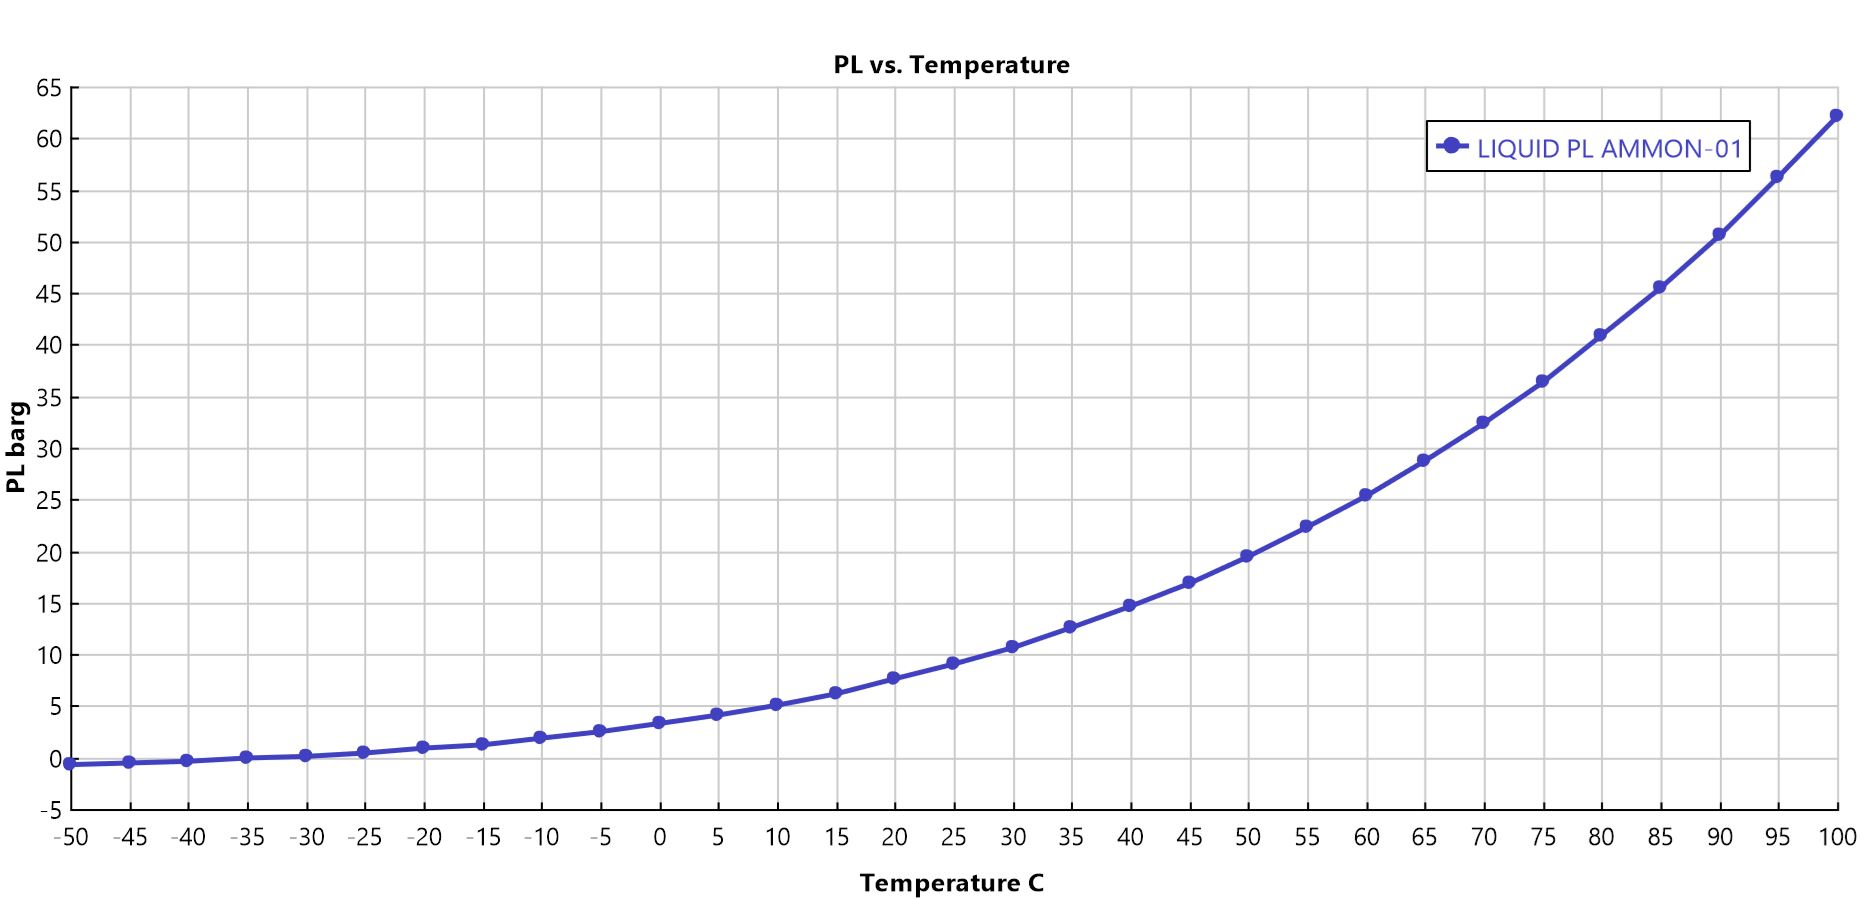
\includegraphics[scale=0.45]{media/PL_vs_temperature.jpg}
	\caption{Graphe de la tension de vapeur (en \unit{}{\bbar g})
	par rapport à la température (en \unit{}{\degreecelsius}).}
	\label{pvst}
\end{figure}

\begin{figure}[htb!]
	\centering
	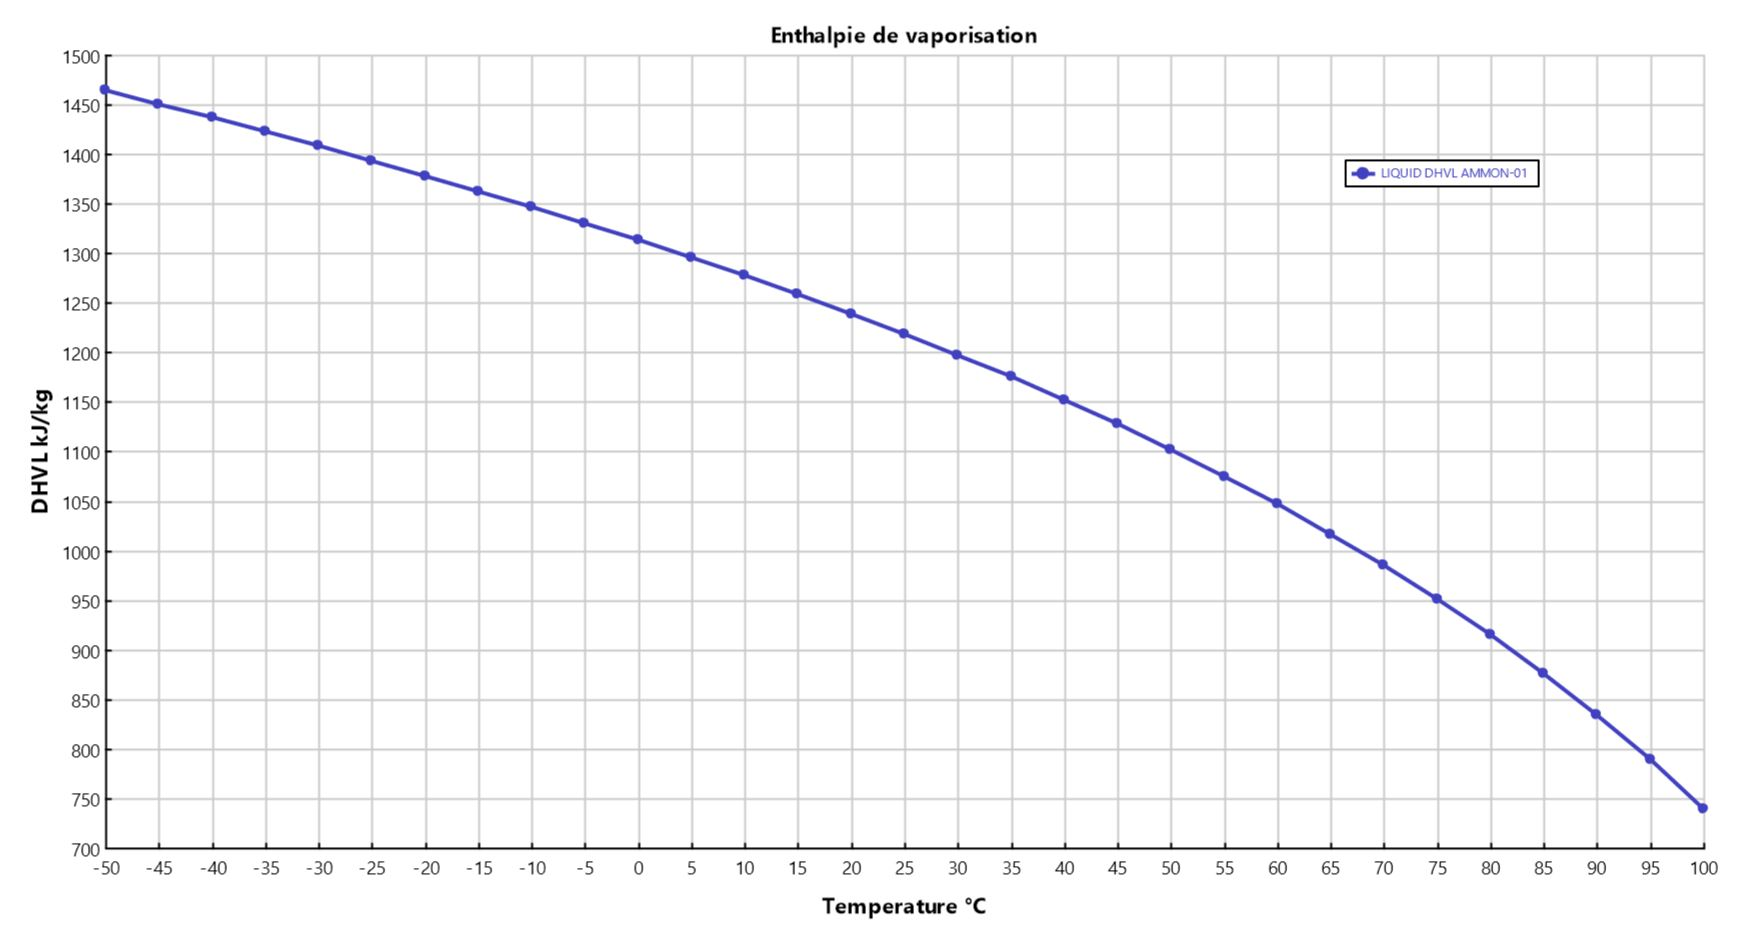
\includegraphics[scale=0.49]{media/enthalpie_vap.jpg}
	\caption{Graphe de l'enthalpie de vaporisation 
	(en \unit{}{\kilo\joule\per\kilo\gram}) par rapport à
	la température (en \unit{}{\degreecelsius}).}
	\label{vap}
\end{figure}

\section{Questions}
\paragraph{Quelle est la pression normale de stockage?}
La température normale de stockage étant de \unit{20}{\degreecelsius}
et la pression à l'intérieur du tank étant égale à la tension
de vapeur de l'ammoniac, on trouve, via la figure
\ref{pvst} 

$$p_{\text{normale}} \approx \unit{8}{\bbar g} = \unit{9}{\bbar}.$$

\paragraph{Quelle sera la pression de stockage en été 
(\unit{30}{\degreecelsius})?}
A nouveau, en s'aidant de la figure \ref{pvst}, on trouve

$$p_{\text{été}} \approx \unit{11}{\bbar g} = \unit{12}{\bbar}.$$

\paragraph{Quelle sera la pression maximale de tarage
de la soupape de sécurité?}
La pression maximale de tarage est égale à la pression de 
design du tank, c'est à dire

$$p_{\text{tarage, max}} = \unit{15}{\bbar g} = \unit{16}{\bbar}.$$

Pour les trois questions suivantes, on considère la pression
de tarage de la soupape comme étant égale à \unit{16}{\bbar}.

\paragraph{Quelle sera la pression durant la décharge?}
Dans le cas d'un incendie, la surpression autorisée est de 121\%
de la pression de tarage \cite{mignon}, à savoir 

$$p_{\text{décharge}} = \unit{19.36}{\bbar}$$

dans notre cas.

\paragraph{Quelle sera la température du liquide durant
la décharge via la soupape?}
A partir de le figure \ref{pvst}, on trouve 

$$T \approx \unit{49.5}{\degreecelsius} = \unit{322.65}{\kelvin}.$$

\paragraph{Quelle sera la taille de la soupape nécessaire?}
La taille de l'orifice de la soupape se calcule en utilisant la formule
suivante\cite{mignon} 

$$A = \frac{W}{CK_dP_1K_bK_c}\sqrt{\frac{TZ}{M}}.$$

Afin d'y voir plus clair, listons dans un premier temps 
tous les paramètres connus et convertissons, si nécessaire,
leurs unités selon les besoins de la formule.

\begin{itemize}
	\item $K_d$ est le coéfficient de décharge. Pour un gaz,
	on a $K_d = 0.975$ ;
	\item $P_1$ est la préssion durant la décharge, on a donc
	$P_1 = p_{\text{décharge}} = \unit{19.36}{\bbar} = 
	\unit{19.36\cdot10^2}{\kilo\pascal}$ ;
	\item $K_b$ est un facteur de correction dû à contrepression. 
	Sa valeur pour une soupape conventionnelle comme la nôtre est de 1 ;
	\item $K_c$ est un facteur de correction dû aux éventuelles
	combinaisons soupape/disque de rupture. Dans notre cas, $K_c = 1$ ;
	\item $T$ est la témpérature de décharge, c'est à dire 
	\unit{322.65}{\kelvin} ;
	\item $Z = 1$ ;
	\item $M$ est la masse moléculaire, on calculer assez 
	simplement que $M = \unit{17}{\kilo\gram\per\kilo\mole}$.
\end{itemize}

% FIXME : c'est quoi C ?
Occupons-nous maintenant des paramètres inconnus : $C$ et $W$,
qui est débit massique relâché.
La premier peut être calculé à partir de la formule suivante\cite{mignon}

$$C = 0.03948\sqrt{k\frac{2}{k+1}^{\frac{k+1}{k-1}}}$$

où $k = \frac{C_p}{C_v} = 1.33$. On a donc $C = 0.02655536953$.

Le deuxième est un petit peu plus compliqué à obtenir. Pour obtenir
$W$, nous allons utiliser la formule suivante\cite{mignon}

$$W = \frac{Q}{\Delta H_{\text{vap}}(T_{\text{décharge}})}$$ 

où $\Delta H_{\text{vap}}(T_{\text{décharge}}) \approx 
\unit{1115\cdot10^3}{\joule\per\kilo\gram}$ est trouvé en utilisant
la figure \ref{vap}. Pour calculer $Q$, qui correspond à
l'absorption totale de chaleur par les surfaces en contact avec
l'ammoniac liquide (exprimé en \unit{}{\watt}) nous pouvons
utiliser la formule suivante\cite{mignon}

$$Q = C_1FA_{\text{ws}}^{0.82}$$

où $C_1 = 43200$ est une constante, $F$ est un 
facteur d'environnement et $A_{\text{ws}}$ correspond
à l'aire de la \textit{wetted surface}, autrement dit
il s'agit de la surface totale en contact avec l'ammoniac
liquide. On peut trouver la valeur de $F$ dans des tables
\cite{mignon}. Dans notre cas, le tank n'étant pas isolé,
on trouve $F = 1.0$.

Calculons maintenant $A_{\text{ws}}$. Avant tout, il faut
savoir qu'on considère qu'il n'y a plus d'absorption de chaleur
à \unit{7.62}{\meter} au dessus du feu\cite{mignon}.
$A_{\text{ws}}$ est constitué de deux surfaces ; la partie
basse du tank constitué de l'hémisphère et la partie centrale
constitué du cylindre. L'hémisphère de rayon égale à \unit{3}{\meter}
a une surface de \unit{56.54866776}{\meter\squared} et la partie
cylindrique d'une hauteur de \unit{4.62}{\meter} a une surface
de \unit{87.08494836}{\meter\squared}. On a donc finalement 
$A_{\text{ws}} = \unit{143.6336161}{\meter\squared}$.

On trouve dès lors que $Q = \unit{2537661.812}{\watt}$.
On fini enfin par obtenir 

$$W = \unit{2.275929876}{\kilo\gram\per\second} =
\unit{8193.347554}{\kilo\gram\per\hour}.$$

Nous disposons maintenant de toutes les informations nécessaires
pour calculer $A$ :

$$A = \unit{712.0990948}{\milli\meter\squared}.$$

La soupape standard correspondantes à cette aire est une soupape
de modèle J\cite{mignon}.

\paragraph{Si la pression de design de l'équipement était de \unit{20}{\bbar g},
quel serait l'effet d'augmenter la pression de tarage de \unit{5}{\bbar} et de 
la porter à \unit{20}{\bbar g}?}
Afin d'éviter de refaire tous les calculs (et les divers changement d'unités)
pouvant aboutir à un grand nombre d'erreurs de calculs et de conversion, nous
avons créer une fonction Matlab permettant de calculer la taille de l'orifice
automatiquement (présente en annexe \ref{code-matlab}. Cette fonction prend 4 paramètres en argument : la pression
de tarage en bars absolu, la température de décharge en Kelvin (mesurable sur
la figure \ref{pvst}), l'enthalpie de vaporisation correspondant
à la température de décharge en kilojoules (mesurable sur la figure \ref{vap}) et un dernier
paramètre dont la valeur vaut 1 pour cette question\footnote{Ce paramètre $F$ dépend
de l'isolement thermique du réservoir, ici on suppose qu'il n'est pas isolé.}.
Dans ca cas ci, la pression de tarage vaut \unit{21}{\bbar}. La pression
de décharge valant, dans le cas d'un incendie, 121\% de ma pression de tarage,
on peut trouver la température de décharge et l'enthalpie de vaporisation
correspondante. On trouve $T_{\text{décharge}} = \unit{58}{\degreecelsius}$
et $\Delta H_{\text{vap}}(T_{\text{décharge}}) = \unit{1050}{\kilo\joule\per\kilo\gram}$.
En rentrant ces 3 paramètres dans notre fonction, on trouve 

$$A = \unit{578.06}{\milli\meter\squared}.$$

La soupape standard correspondante à cette aire est également
un modèle J\cite{mignon}.

\paragraph{Pour la première pression de tarage, quelle est l'influence
d'isoler thermiquement le tank avec un isolant tel que le coefficient
d'échange avec l'extérieur soit réduit à une valeur de
\unit{10}{\watt\per\meter\squared\kelvin}?}
En cherchant dans une table qui fait la correspondance 
entre le coéfficient d'échange avec l'extérieur et la valeur
de $F$ utilisée dans le calcul de $Q$, on trouve, pour un
coéfficient de 11.36 que $F$ vaut 0.15. On peut donc
réutiliser notre fonction Matlab en ajoutant ce paramètre.
On obtient 

$$A = \unit{103.463}{\milli\meter\squared}$$

soit presque 7 fois moins que sans isolation thermique.
La soupape standard correspondante à cette aire est le modèle
1E2.

\biblio{sources-tache5}
\appendix
\section{Code Matlab utilisé}
\label{code-matlab}
\lstinputlisting{matlab/SizePSV.m}
\end{document}
